\chapter{软间隔最大化和线性支持向量机}

\section{线性支持向量机}

假定给定一个特征空间的训练数据集
\begin{equation}
    T=\{(x_1,y_1),(x_2,y_2),\cdots,(x_N,y_N)\}
\end{equation}

其中$x_i\in \mathbb{R}^n$,$y_i={-1,+1},i=1,2,\cdots,N$,其中$x_i$为第$i$个特征向量。通常情况下,
训练数据中有一些\textsl{特异点(outlier)},将这些特异点除去后,剩下大部分的样本点的集合是线性可分的。

线性不可分意味着某些样本点$(x_i,y_i)$不能满足函数间隔大于等于1的约束条件。为了解决这个问题,可以对每个样本点
$(x_i,y_i)$引进一个松弛变量$\xi_i\leqslant 0$,使得函数间隔加上松弛变量大于等于$1$,这样约束条件变为
\begin{equation}
    y_i(\omega\cdot x_i+b)\geqslant 1-\xi_i
\end{equation}

同时对每个松弛变量$\xi_i$,支付一个代价$\xi_i$,目标函数由由原来的$\frac{1}{2}\Vert \omega\Vert^2$变成
\begin{equation}
    \frac{1}{2}\Vert\omega\Vert^2+C\sum\limits_{i=1}^{N} \xi_i
\end{equation}

其中$C>0$称为\textbf{\textsl{惩罚参数}}。$C$值大时对误分类的惩罚增大,反之惩罚减小。

\subsection*{线性支持向量机的定义}
\begin{define}
    对于给定的线性不可分的训练数据集,通过求解以下凸二次规划问题(原始问题)
    \begin{equation}
        \begin{aligned}
            & \min\limits_{\omega,b,\xi}\ \  \frac{1}{2}\Vert\omega\Vert^2+C\sum\limits_{i=1}^{N}\xi_i\\
            & s.t. \ \ \ y_i(\omega\cdot x_i+b)\geqslant 1-\xi_i,\ \ i=1,2,\cdots,N\\
            & \ \ \ \ \ \ \ \ \ \xi_i\geqslant 0,\ \ i=1,2,\cdots,N
        \end{aligned}
    \end{equation}

    即软间隔最大化问题,得到的分离超平面为
    \begin{equation}
        \omega^*\cdot x+b^*=0
    \end{equation}

    以及相应的分类决策函数
    \begin{equation}
        f(x)=sign(\omega^*\cdot x+b^*)
    \end{equation}

    称为\textsl{\textbf{线性支持向量机}}。
\end{define}

\section{学习的对偶问题}

原始问题的拉格朗日函数为

\begin{equation}
    L(\omega,b,\xi,\alpha,\mu)=\frac{1}{2}\Vert\omega\Vert^2+C\sum\limits_{i=1}^{N}\xi_i
    -\sum\limits_{i=1}^{N}\alpha_i(y_i(\omega\cdot x_i+b)-1+\xi_i)-\sum\limits_{i=1}^{N}
    \mu_i\xi_i
\end{equation}

其中$\alpha_i\geqslant 0,\mu_i\geqslant 0$。

对偶问题时拉格朗日函数的极大极小值问题,首先对$L(\omega,b,\xi,\alpha,\mu)$求极小

\begin{eqnarray}
    & \nabla_\omega L(\omega,b,\xi,\alpha,\mu)=\omega-\sum\limits_{i=1}^{N}\alpha_iy_ix_i=0\\
    & \nabla_b L(\omega,b,\xi,\alpha,\mu) = -\sum\limits_{i=1}^{N} \alpha_iy_i=0\\
    & \nabla_{\xi_i} L(\omega,b,\xi,\alpha,\mu)=C-\alpha_i-\mu_i=0
 \end{eqnarray}

 求解得到
 \begin{eqnarray}
    & \omega=\sum\limits_{i=1}^{N} \alpha_iy_ix_i\\
    & \sum\limits_{i=1}^{N}\alpha_iy_i=0\\
    & C-\alpha_i-\mu_i=0
 \end{eqnarray}

 代入拉格朗日函数得到

 \begin{equation}
    \min\limits_{\omega,b,\xi} L(\omega,b,\xi,\alpha,\mu)=-\frac{1}{2}\sum\limits_{i=1}^{N}
    \sum\limits_{j=1}^{N}\alpha_i\alpha_jy_iy_j(x_i\cdot x_j)+\sum\limits_{i=1}^{N}\alpha_i
\end{equation}

再对极小问题求极大,即得到对偶最优化问题

\begin{eqnarray}
    & \max\limits_{\alpha} &-\frac{1}{2}\sum\limits_{i=1}^{N}\sum\limits_{j=1}^{N}\alpha_i\alpha_j(x_i\cdot x_j)+\sum\limits_{i=1}^{N}\alpha_i\\
    & s.t. & \sum\limits_{i=1}^{N}\alpha_iy_i=0\\
    & & C-\alpha_i-\mu_i=0 \label{eq:7.46}\\
    & & \alpha_i\geqslant 0\\
    & & \mu_i\geqslant 0,\ \ i=1,2,\cdots,N
\end{eqnarray}

将对偶最优化问题进行变换,利用等式约束(\ref{eq:7.46})消去$\mu_i$,从而只留下变量$\alpha_i$,并将对目标函数求极小转换为求极大。即得到原始问题的对偶问题是
\begin{framed}

\begin{eqnarray}
    & \min\limits_{\alpha} \ \ &\frac{1}{2}\sum\limits_{i=1}^{N}\sum\limits_{j=1}^{N}
    \alpha_i\alpha_jy_iy_j(x_i\cdot x_j)-\sum\limits_{i=1}^{N}\alpha_i\\
    & s.t. & \sum\limits_{i=1}^{N}\alpha_iy_i=0\\
    &      & 0\leqslant \alpha_i\leqslant C,\ \ i=1,2,\cdots,N
\end{eqnarray}
    
\end{framed}

可以通过求解对偶问题而得到原始问题的解,进而确定分离超平面和决策函数。

\subsection*{原始问题最优解和对偶问题最优解的关系}

\begin{theorem}
    设$\alpha^*=(\alpha^*_1,\alpha^*_2,\cdots,\alpha^*_N)^T$是对偶问题的一个解,若存在$\alpha^*$的一个分量
    $a^*_j(0 <\alpha^*<C)$,则原始问题的解$\omega^*,b^*$可按照下式求得
    \begin{eqnarray}
        & \omega=\sum\limits_{i=1}^{N}\alpha^*_iy_ix_i\\
        & b^* = y_i-\sum\limits_{i=1}^{N}y_i\alpha^*(x_i\cdot x_j)
    \end{eqnarray}
\end{theorem}
\textbf{proof. } 原始问题是凸二次规划问题,解满足KKT条件,
\begin{eqnarray}
    & \nabla_\omega L(\omega^*,b^*,\xi^*,\alpha^*,\mu^*)=\omega^*-\sum\limits_{i=1}^{N}\alpha^*y_ix_i=0\\
    & \nabla_b L(\omega^*,b^*,\xi^*,\alpha^*,\mu^*) = -\sum\limits_{i=1}^{N}\alpha^*y_i=0\\
    & \nabla_\xi L(\omega^*,b^*,\xi^*,\alpha^*,\mu^*) = C-\alpha^*-\mu^*=0\\
    & \alpha_i^*(y_i(\omega^*\cdot x_i+b^*)-1+\xi^*_i)=0\\
    & \mu^*_i\xi^*_i = 0\\
    & y_i(\omega^*\cdot x_i+b^*)-1+\xi^*_i\geqslant 0\\
    & \xi^*_i\geqslant 0\\
    & \alpha^*_i\geqslant 0\\
    & \mu^*_i\geqslant 0,\ \ i=1,2,\cdots,N
\end{eqnarray}

由此定理可知,分离超平面可以写成
\begin{equation}
    \sum\limits_{i=1}^{N} \alpha^*_iy_i(x\cdot x_i)+b^*=0
\end{equation}

分类决策函数可以写成
\begin{equation}
    f(x)=sign(\sum\limits_{i=1}^{N} \alpha^*_iy_i(x\cdot x_i)+b^*)
\end{equation}

上式子称为\textsl{\textbf{线性支持向量机的对偶形式}}。

\section{线性支持向量机学习算法}

输入:训练数据集$T=\{(x_1,y_1),(x_2,y_2),\cdots,(x_N,y_N)\}$,其中$x_i\in \mathbb{R}^n$,$y_i=\{-1,+1\}$。

输出:分离超平面和决策函数。

\begin{enumerate}[itemindent=2em]
    \item 选择惩罚参数$C>0$,构造并求解凸二次规划问题
    \begin{eqnarray}
        & \min\limits_{\alpha} \ \ &\frac{1}{2}\sum\limits_{i=1}^{N}\sum\limits_{j=1}^{N}
        \alpha_i\alpha_jy_iy_j(x_i\cdot x_j)-\sum\limits_{i=1}^{N}\alpha_i\\
        & s.t. & \sum\limits_{i=1}^{N}\alpha_iy_i=0\\
        &      & 0\leqslant \alpha_i\leqslant C,\ \ i=1,2,\cdots,N
    \end{eqnarray}

    求得最优解$\alpha^*=(\alpha^*_1,\alpha^*_2,\cdots,\alpha^*_N)^T$。
    \item 计算$\omega^*=\sum\limits_{i=1}^{N}\alpha^*_iy_ix_i$。选择$\alpha^*$的一个分量$\alpha^*_j$适合条件$0<\alpha^*_j<C$,计算
    \begin{equation}
        b^*=y_i-\sum\limits_{i=1}^{N}y_i\alpha^*_i(x_i\cdot x_i)
    \end{equation}
\end{enumerate}

求得分离超平面和决策函数
\begin{eqnarray}
    & \omega^*\cdot x+b^*=0\\
    & f(x)=sign(\omega^*\cdot x+b^*)
\end{eqnarray}

从理论上,原始问题对$b$的解可能不唯一,然而实际应用中,往往只会出现算法叙述的情况。

\section{支持向量}

在线性不可分的情况下,将对偶问题的解$\alpha^*=(\alpha^*_1,\alpha^*_2,\cdots,\alpha^*_N)$中对应
$\alpha^*_i>0$的样本点$(x_i,y_i)$的实例$x_i$称为\textsl{\textbf{软间隔的支持向量}}。

\begin{figure}[H]
    \centering
    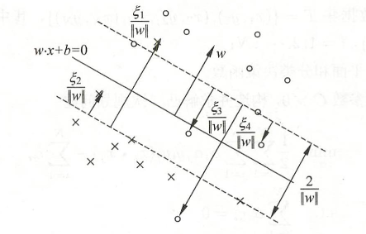
\includegraphics[scale=0.6]{figures/软间隔的支持向量.png}
    \caption{软间隔的支持向量}
    \label{软间隔的支持向量}
\end{figure}

如上图所示,分离超平面由实线表示,间隔边界由虚线表示,正例点由”$\circ$“表示,负例点由$\times$表示。图中还标出了实例$x_i$到间隔
边界的距离$\frac{\xi_i}{\Vert\omega\Vert}$。

软间隔的支持向量$x_i$或者在间隔边界上,或者在间隔边界与分离超平面之间,或者在分离超平面误分一侧。
\begin{enumerate}[itemindent=2em]
    \item 若$\alpha^*_i<C$,则$\xi_i=0$,支持向量$x_i$恰好活在间隔边界上;
    \item 若$\alpha^*_i=C$,$0<\xi_i<1$,则分类正确,$x_i$在间隔边界与分离超平面之间;
    \item 若$\alpha^*_i=C$,$\xi_i=1$,则$x_i$在分离超平面上;
    \item 若$\alpha^*_i=C$,$\xi_i>1$,则$x_i$位于分离超平面误分一侧。
\end{enumerate}


\section{合页损失函数}

线性支持向量机学习还有另一种解释,就是最小化以下目标函数
\begin{equation}
    \sum\limits_{i=1}^{N}[1-y_i(\omega\cdot x_i+b)]_{+}+\lambda\Vert\omega\Vert^2
\end{equation}

目标函数的第1项是经验损失或经验风险,函数
\begin{equation}
    L(\omega\cdot x+b)=[1-y_i(\omega\cdot x_i+b)]_{+}
\end{equation}

称为\textsl{\textbf{合页损失函数}(hinge loss function)}。下标"+"表示一下正值函数
\begin{equation}
    |z|_+=\begin{cases}
        & z, \ \ \ z>0\\
        & 0, \ \ \ z\leqslant 0 
    \end{cases}
\end{equation}

即当样本点被正确分类且函数间隔(确信度)$y_i(\omega\cdot x_i+b)$大于1时,损失为0。否则损失是
$1-y_i(\omega\cdot x_i+b)$。注意到图(\ref{软间隔的支持向量})中的实例点$x_4$被正确分类,
但损失部位0,目标函数的第2项是系数为$\lambda$的$\omega$的$L_2$范数,是正则化项。

\subsection*{线性支持向量机原始问题的等价最优化问题 }
\begin{theorem}
    线性支持向量机的原始最优化问题等价于最优化问题
    \begin{equation}
        \min\limits_{\omega,b}\sum\limits_{i=1}^{N}[1-y_i(\omega\cdot x_i+b)]_{+}+\lambda\Vert\omega\Vert^2
    \end{equation}
\end{theorem}
\textbf{proof. }

\subsection*{合页损失函数的几何意义}
合页损失函数的图形如下图所示
\begin{figure}[H]
    \centering
    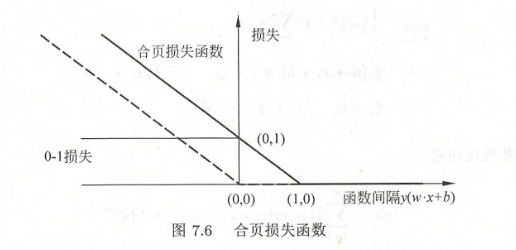
\includegraphics[scale=0.45]{figures/合页损失函数.png}
    \caption{合页损失函数}
    \label{合页损失函数}
\end{figure}

横轴是函数间隔$y(\omega\cdot x+b)$,纵轴是损失\footnote{由于函数形状像一个合页,故称合页损失函数}。

图中还画出\textsl{0-1损失函数}。可以认为他是二分类问题的真正的损失函数,而合页损失函数是0-1损失函数的上界。
由于0-1损失函数不是连续可导的,直接优化由于其构成的目标函数比较困难,可以认为线性支持向量机是优化由0-1损失函数
的上界构成的目标函数。这时的上界损失函数又称为\textsl{\textbf{代理损失函数}(surrogate loss function)}。

图中虚线显示的是感知机的损失函数
\begin{equation}
    [-y_i(\omega\cdot x_i+b)]_+
\end{equation}

这时,当样本点被正确分类时,损失为$0$,否则损失是$-y_i(\omega\cdot x_i+b)$。相比之下,合页损失函数
不仅要求分类正确,且确信度足够高时损失才是$0$,即合页损失函数对学习有更高要求。
